\subsection{Reiterate self-energy requirements}

\begin{frame}
  \frametitle{Reiterate self-energy requirements}
  \tikzset{block/.style={
          shape=rectangle,draw,minimum size=.8cm},
      dd/.style={densely dotted},
      block dd/.style={block,dd},
  }
  \def\bsize{.8cm}

  \begin{block}{Rules for using self-energies}

    Coupling a \emph{bulk} electrode to a device requires(!) coupling region to behave
    \emph{bulk} as well. 

    \vspace{4pt}

    \begin{center}
      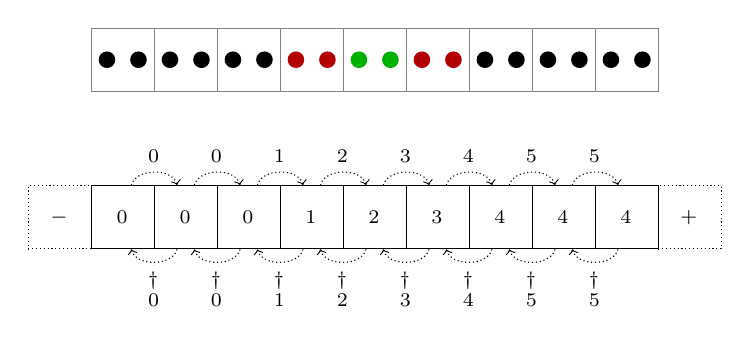
\begin{tikzpicture}

        \foreach \x in {0,1,2,3,4,5,6,7,8} {
            \def\tmpcol{black}
            \ifnum\x>2
            \def\tmpcol{red!70!black}
            \fi
            \ifnum\x>3
            \def\tmpcol{green!70!black}
            \fi
            \ifnum\x>4
            \def\tmpcol{red!70!black}
            \fi
            \ifnum\x>5
            \def\tmpcol{black}
            \fi
            \node[block,gray] at ({(\x-0.5)*\bsize},3*\bsize) {};

            \expandafter\fill\expandafter[\tmpcol] ({(\x-0.75)*\bsize},3*\bsize)
            circle (3pt);
            \expandafter\fill\expandafter[\tmpcol] ({(\x-0.25)*\bsize},3*\bsize)
            circle (3pt);

        }
    
        \node[block dd] at (-1.5*\bsize,0.5*\bsize) {$\SE_{-}$};
        \foreach \x in {0,1,2,3,4,5,6,7,8} {
            \ifnum\x<3
            \def\tmpnum{0}
            \fi
            \ifnum\x>2
            \pgfmathparse{int(\x-2)}
            \edef\tmpnum{\pgfmathresult}
            \fi
            \ifnum\x>5
            \pgfmathparse{int(4)}
            \edef\tmpnum{\pgfmathresult}
            \fi
            \node[block] (A\x) at ({(\x-0.5)*\bsize},0.5*\bsize) {$\HH_\tmpnum$};
            \ifnum\x>0
            \pgfmathparse{int(\x-1)}
            \edef\xp{\pgfmathresult}
            \ifnum\x>6
            \pgfmathparse{int(5)}
            \edef\tmpnum{\pgfmathresult}
            \fi
            \draw[->,dd] (A\xp) to[out=75,in=105] node[above] {$\VV_\tmpnum$} (A\x);
            \draw[<-,dd] (A\xp) to[out=-75,in=-105] node[below] {$\VV^\dagger_\tmpnum$} (A\x);
            \fi
        }
        \node[block dd] at (8.5*\bsize,0.5*\bsize) {$\SE_{+}$};
      \end{tikzpicture}

    \end{center}

    \vspace{-12pt}

    \begin{itemize}
      \item<+-> Remember that $\SE_{-/+}$ is a correction to the Hamiltonian (i.e. 
      $\HH = \HH + \SE$)

      \item \emph{Extremely} important in TranSiesta, electrostatics are long-range!
    \end{itemize}
  \end{block}

  % \begin{block}<2->{Use symmetries whenever you can}

  %   \begin{itemize}
  %     \item If you have transverse periodic electrodes you should apply Bloch's theorem
  %     using the flag \texttt{Bloch}
  %   \end{itemize}
    
  % \end{block}

\end{frame}


%%% Local Variables:
%%% mode: latex
%%% TeX-master: "talk"
%%% End:
